\documentclass[10pt,a4paper]{article}
\usepackage[left=2cm,right=2cm,top=2cm,bottom=2cm]{geometry}
\usepackage[T1]{fontenc}
\usepackage{lmodern}
\usepackage[spanish,es-tabla,es-noquoting]{babel}
\usepackage[dvipsnames]{xcolor}
\usepackage[fleqn]{mathtools}
\usepackage{booktabs}
\usepackage{amsmath}
\usepackage{latexsym}
\usepackage{graphicx}
\usepackage{nccmath}
\usepackage{multicol}
\usepackage{listings}
\usepackage{color}
\usepackage{float}
\usepackage{csquotes}

\definecolor{colorIPN}{rgb}{0.5, 0.0,0.13}
\definecolor{colorESCOM}{rgb}{0.0, 0.5,1.0}
\graphicspath{ {imagenes/} }

\begin{document}
%#########################################################
\begin{titlepage}
	\centering

	{\color{colorIPN}\rule{\linewidth}{1.4pt}}\\[0.35cm]
	{\scshape\LARGE Instituto Politécnico Nacional}\\[0.2cm]
	{\scshape\Large \color{colorESCOM}Escuela Superior de Cómputo}\\[0.35cm]
	{\color{colorIPN}\rule{\linewidth}{0.5pt}}

	\vspace{1.6cm}
	{\large \color{colorESCOM}\MakeUppercase{Administración de Servicios en Red}\par}

	\vspace{2cm}
	\noindent
	\begin{minipage}[t]{0.025\linewidth}
		\color{colorESCOM}\rule{3.2pt}{3.6cm}
	\end{minipage}%
	\hspace{0.5cm}%
	\begin{minipage}[t]{0.87\linewidth}
		\raggedright\huge\bfseries\color{colorIPN} Práctica 1: Instalación y configuración básica de GNS3
	\end{minipage}

	\vspace{2.8cm}
	\renewcommand{\arraystretch}{1.7}
	\begin{tabular}{r @{\hspace{0.6cm}} l}
		{\bfseries\color{colorESCOM}Profesor:} & {\itshape\color{colorIPN} Marco Antonio Tenorio Marrón} \\
		{\bfseries\color{colorESCOM}Alumno:}   & {\itshape\color{colorIPN} Angel Frausto Robles} \\
		{\bfseries\color{colorESCOM}Boleta:}   & {\itshape\color{colorIPN} 2019630177} \\
		{\bfseries\color{colorESCOM}Grupo:}    & {\itshape\color{colorIPN} 7CM3} \\
	\end{tabular}

	\vfill
	{\color{colorIPN}\rule{0.25\linewidth}{0.5pt}}\\[0.25cm]
	{\small\color{colorIPN}\today\par}
	\vspace{1cm}
\end{titlepage}

\renewcommand\lstlistingname{Código}

\lstset{
	basicstyle=\small\ttfamily,
	numbers=left,
	numberstyle=\tiny,
	frame=tb,
	tabsize=4,
	columns=fixed,
	showstringspaces=false,
	showtabs=false,
	keepspaces,
	commentstyle=\color{Violet},
	keywordstyle=\color{colorIPN} \bfseries,
	stringstyle=\color{colorESCOM},
	breaklines=true,
	extendedchars=true,
	inputencoding=utf8,
	literate=
		{á}{{\'a}}1 {é}{{\'e}}1 {í}{{\'i}}1 {ó}{{\'o}}1 {ú}{{\'u}}1
		{Á}{{\'A}}1 {É}{{\'E}}1 {Í}{{\'I}}1 {Ó}{{\'O}}1 {Ú}{{\'U}}1
		{ñ}{{\~n}}1 {Ñ}{{\~N}}1 {ü}{{\"u}}1 {¿}{{?`}}1 {¡}{{!`}}1
}

\pagenumbering{arabic}

%################################################
\section{\color{colorIPN}{Objetivo}}

Instalar y configurar GNS3 como entorno de simulación de red, y construir en él una topología mínima de dos redes separadas interconectadas por un router, para comprobar el direccionamiento IP y el ruteo básico entre ambas.

%################################################
\section{\color{colorIPN}{Topología}}

La práctica interconecta dos redes de área local a través de un router con dos interfaces FastEthernet. Cada red tiene un equipo terminal conectado a un switch de capa 2, y el switch se conecta a una interfaz distinta del router:

\begin{table}[H]
	\centering
	\begin{tabular}{@{}llll@{}}
		\toprule
		Dispositivo & Interfaz & Dirección IP & Conecta a \\
		\midrule
		PC1 & Ethernet0 & 10.10.1.10 /24 & Switch1 \\
		Switch1 & -- & -- & PC1, R1 (Fa0/0) \\
		R1 (router C3660) & FastEthernet0/0 & 10.10.1.1 /24 & Switch1 \\
		R1 (router C3660) & FastEthernet1/0 & 10.10.2.1 /24 & Switch2 \\
		Switch2 & -- & -- & R1 (Fa1/0), PC2 \\
		PC2 & Ethernet0 & 10.10.2.10 /24 & Switch2 \\
		\bottomrule
	\end{tabular}
	\caption{Direccionamiento de la topología}
	\label{tab:direccionamiento}
\end{table}

\begin{figure}[H]
	\centering
	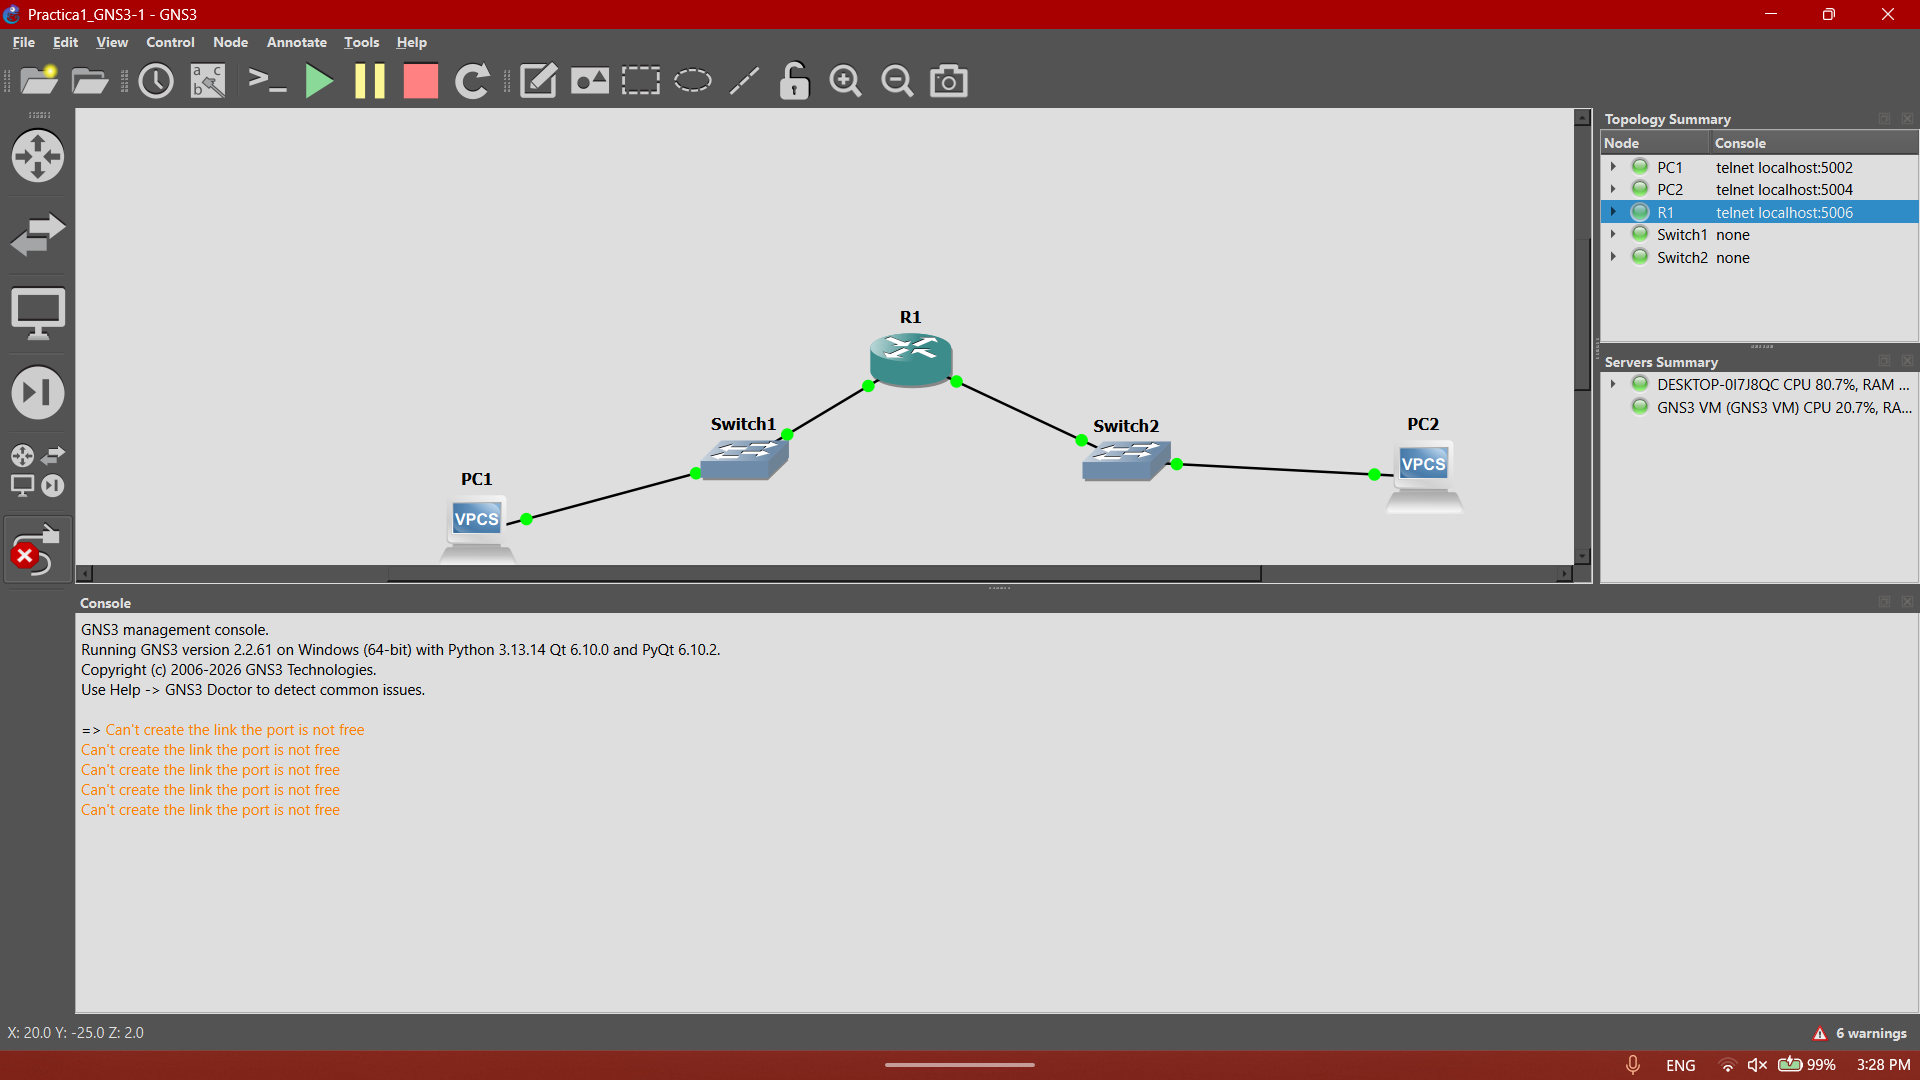
\includegraphics[width=0.95\linewidth]{00_topologia_completa.png}
	\caption{Topología completa en GNS3: PC1 — Switch1 — R1 — Switch2 — PC2, todos los dispositivos en ejecución}
	\label{img:topologia}
\end{figure}

%################################################
\section{\color{colorIPN}{Desarrollo}}

\subsection{\color{colorESCOM}{Instalación de GNS3}}

Se instaló GNS3 (versión 2.2.61) desde el instalador oficial \texttt{GNS3-2.2.61-all-in-one.exe}, junto con la GNS3 VM sobre VirtualBox para el soporte de dispositivos que no pueden correr de forma nativa en Windows.

\subsection{\color{colorESCOM}{Router y módulos}}

GNS3 no distribuye imágenes IOS de Cisco por motivos de licencia, así que la imagen se importó por separado (\texttt{c3660-a3jk9s-mz.124-25d.bin}) mediante \textit{Edit > Preferences > Dynamips > IOS routers > New}. Se configuró un router \textbf{C3600, chasis 3660}, con dos módulos de red para obtener las dos interfaces FastEthernet que pide la topología:

\begin{itemize}
	\item \textbf{Slot 0: Leopard-2FE} — módulo integrado de 2 puertos, provee FastEthernet0/0 y FastEthernet0/1 (esta última sin usar).
	\item \textbf{Slot 1: NM-1FE-TX} — módulo de 1 puerto adicional, provee FastEthernet1/0.
\end{itemize}

\subsection{\color{colorESCOM}{Configuración del router (R1)}}

Con los cuatro enlaces de la topología conectados (PC1--Switch1, Switch1--R1 Fa0/0, R1 Fa1/0--Switch2, Switch2--PC2), se accedió a la consola de R1 y se configuraron las dos interfaces:

\begin{lstlisting}[language=bash, caption={Configuración de las interfaces de R1}]
enable
configure terminal
hostname R1
interface FastEthernet0/0
 ip address 10.10.1.1 255.255.255.0
 no shutdown
exit
interface FastEthernet1/0
 ip address 10.10.2.1 255.255.255.0
 no shutdown
exit
end
write memory
\end{lstlisting}

Ambas interfaces subieron correctamente (\texttt{up/up}) y la configuración se guardó en la NVRAM con \texttt{write memory}.

\subsection{\color{colorESCOM}{Configuración de las PCs (VPCS)}}

Cada PC es un nodo VPCS (Virtual PC Simulator), configurado con su IP, máscara y puerta de enlace en un solo comando:

\begin{lstlisting}[language=bash, caption={Configuración de PC1 y PC2}]
# En PC1
ip 10.10.1.10 255.255.255.0 10.10.1.1

# En PC2
ip 10.10.2.10 255.255.255.0 10.10.2.1
\end{lstlisting}

\begin{figure}[H]
	\centering
	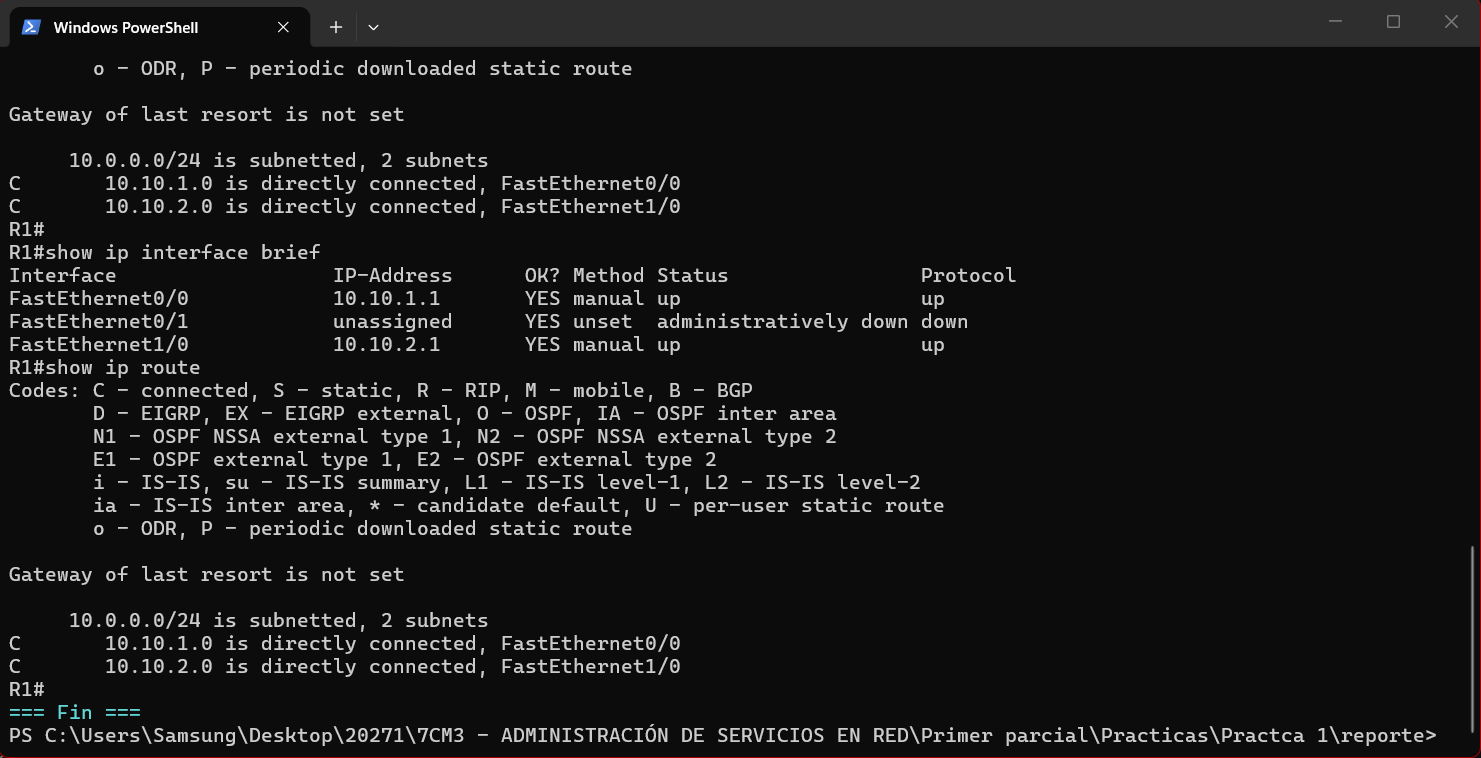
\includegraphics[width=0.95\linewidth]{01_router_interfaces_y_rutas.png}
	\caption{Verificación en R1: \texttt{show ip interface brief} y \texttt{show ip route} tras la configuración}
	\label{img:router-verif}
\end{figure}

\subsection{\color{colorESCOM}{Prueba de conectividad}}

Con las dos PCs configuradas, se verificó la comunicación extremo a extremo entre las dos redes con un \texttt{ping} desde PC1 hacia PC2:

\begin{figure}[H]
	\centering
	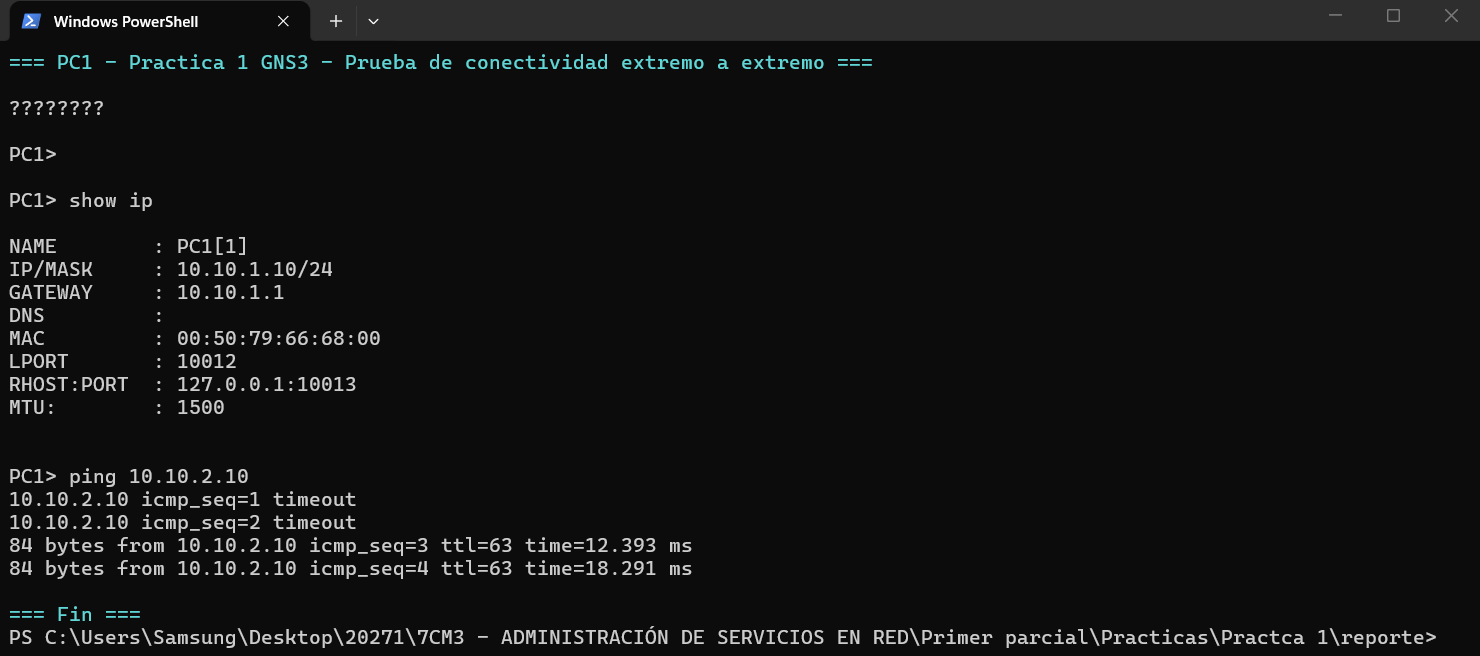
\includegraphics[width=0.95\linewidth]{02_pc1_ip_y_ping_a_pc2.png}
	\caption{IP de PC1 (\texttt{show ip}) y \texttt{ping} exitoso hacia PC2 (10.10.2.10)}
	\label{img:ping}
\end{figure}

El ping llega con \texttt{TTL=63} (en vez de 64), lo que confirma que el paquete atravesó un salto de ruteo, es decir, pasó por R1 en vez de llegar de forma directa: las dos PCs están en subredes distintas (10.10.1.0/24 y 10.10.2.0/24) y solo pueden comunicarse a través del router.

%################################################
\section{\color{colorIPN}{Preguntas}}

\subsection*{\color{colorESCOM}{1. ¿Cuáles son los comandos para entrar al modo EXEC privilegiado y al modo de configuración global?}}

Desde el modo EXEC usuario (\texttt{R1>}), el comando \texttt{enable} entra al modo EXEC privilegiado (\texttt{R1\#}), que da acceso a comandos de administración y verificación. Desde ahí, \texttt{configure terminal} entra al modo de configuración global (\texttt{R1(config)\#}), donde se aplican los cambios de configuración del dispositivo.

\subsection*{\color{colorESCOM}{2. ¿Cuáles son los comandos para asignar una IP a una interfaz y habilitarla? ¿Cuál es el comando completo para FastEthernet 1/0?}}

Dentro del modo de configuración de interfaz, \texttt{ip address \textit{dirección máscara}} asigna la IP y la máscara de subred; por defecto toda interfaz nace administrativamente apagada, así que \texttt{no shutdown} es el comando que la habilita. El comando completo usado para FastEthernet1/0 fue:

\begin{lstlisting}[language=bash]
interface FastEthernet1/0
 ip address 10.10.2.1 255.255.255.0
 no shutdown
\end{lstlisting}

\subsection*{\color{colorESCOM}{3. ¿Cuál es el comando para ver la tabla de ruteo, y de qué tipo son esas rutas?}}

El comando es \texttt{show ip route}. En la tabla de R1 (figura \ref{img:router-verif}) aparecen dos rutas, ambas marcadas con la letra \textbf{C}, es decir, \textbf{directamente conectadas}: el router las aprende automáticamente en cuanto una interfaz con IP asignada pasa a estado \texttt{up/up}, sin necesidad de configurar ningún protocolo de ruteo.

\begin{lstlisting}[language=bash]
C    10.10.1.0 is directly connected, FastEthernet0/0
C    10.10.2.0 is directly connected, FastEthernet1/0
\end{lstlisting}

%################################################
\section{\color{colorIPN}{Conclusiones}}

La topología quedó funcional de extremo a extremo: PC1 y PC2, en dos subredes distintas, se comunican a través de R1 sin necesidad de ningún protocolo de ruteo dinámico, porque ambas rutas son directamente conectadas. La dificultad principal no fue de configuración sino de las imágenes IOS: GNS3 no las incluye por licencia, así que fue necesario conseguir e importar por separado la imagen del C3660, y elegir los módulos de red correctos (Leopard-2FE y NM-1FE-TX) para que las interfaces del router coincidieran exactamente con las que pedía la topología (Fa0/0 y Fa1/0, en dos slots distintos en vez de dos puertos del mismo módulo).

\end{document}
